%%%%%%%%%%%%%%%%%%%%%%%%%%%%%%%%%%%%%%%%%%%%%%%%%%%%%%%%%%%%%%%%%%%%%%%%%%%%%%%%%%%%%%%%%%%%
\chapter{Systèmes du second ordre\label{annexe-2nd}}
%%%%%%%%%%%%%%%%%%%%%%%%%%%%%%%%%%%%%%%%%%%%%%%%%%%%%%%%%%%%%%%%%%%%%%%%%%%%%%%%%%%%%%%%%%%%
\newpage

%%%%%%%%%%%%%%%%%%%%%%%%%%%%%%%%%%%%%%%%%%%%%%%%%%%%%%%%%%%%%%%%%%%%%%%%%%%%%%%%%%%%%%%%%%%%
\section{Abaques}
%%%%%%%%%%%%%%%%%%%%%%%%%%%%%%%%%%%%%%%%%%%%%%%%%%%%%%%%%%%%%%%%%%%%%%%%%%%%%%%%%%%%%%%%%%%%


\paragraph{Dépassement}
\begin{figure}[!h]
\begin{center}
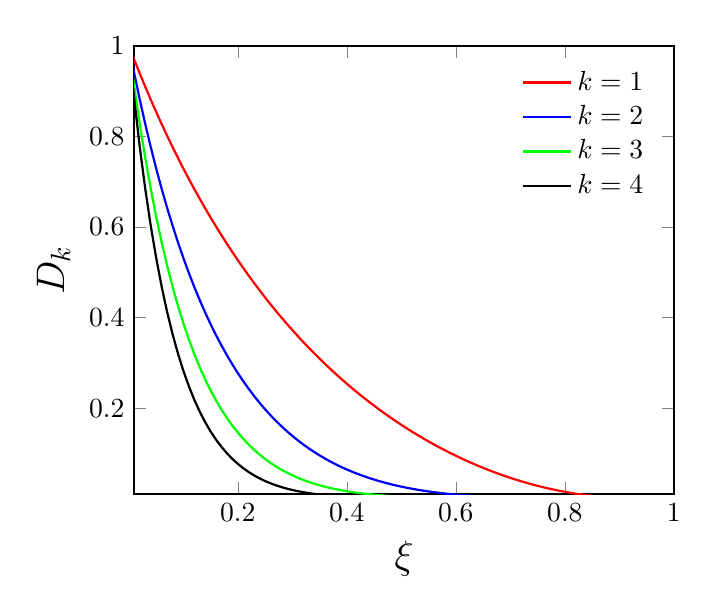
\begin{tikzpicture}
        \pgfmathsetmacro{\pi}{3.141592653589793}     % dépassement d4 
        \begin{axis}[
        %    xmode=log,
        %    ymode=log,
        legend style={draw=none},
        legend pos=north east,
        axis line style = thick,
        xmin=0.01,
        xmax=1,
        ymin=0.01,
        ymax=1.0,
        xlabel={$\xi$},
        ylabel={$D_k$},
        label style={font=\Large},
        ]
\addplot[thick,color=red,domain=0.0001:1, samples=101,unbounded coords=jump]{exp(-(x*\pi)/(sqrt(1-x*x)))};
\addplot[thick,color=blue,domain=0.0001:1, samples=101,unbounded coords=jump]{exp(-(2*x*\pi)/(sqrt(1-x*x)))};
\addplot[thick,color=green,domain=0.0001:1, samples=101,unbounded coords=jump]{exp(-(3*x*\pi)/(sqrt(1-x*x)))};
\addplot[thick,color=black,domain=0.0001:1, samples=101,unbounded coords=jump]{exp(-(4*x*\pi)/(sqrt(1-x*x)))};
\legend{$k=1$,$k=2$,$k=3$,$k=4$}
\end{axis}
\end{tikzpicture}
\end{center}
\end{figure}

\paragraph{Temps de réponse à 5\%}

\begin{figure}[!hb]
    \centering
    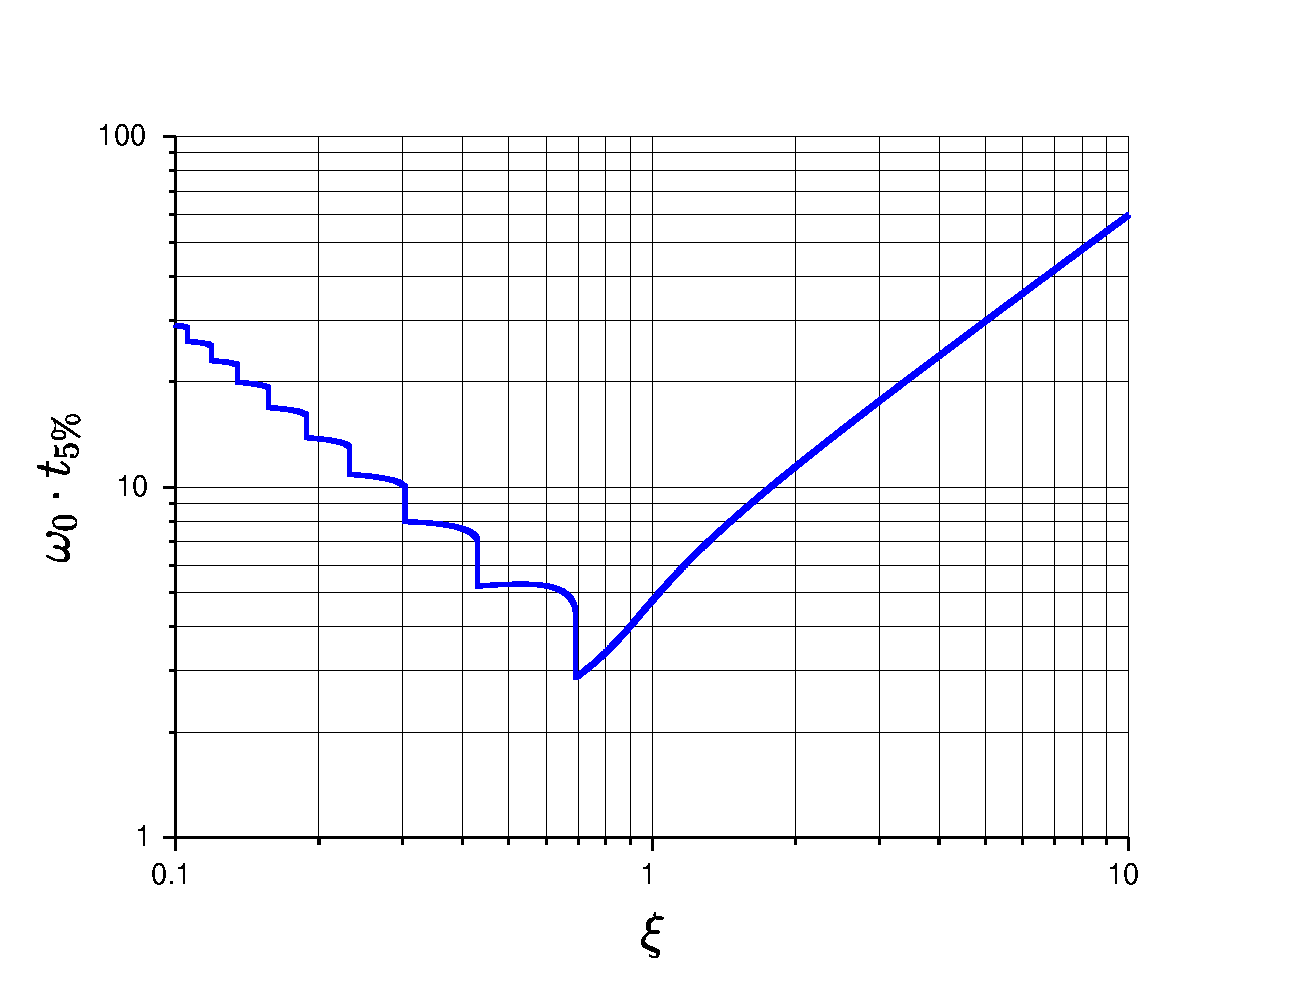
\includegraphics[width=0.8\textwidth]{script/fig_temps_de_reduit.eps}
\end{figure}
\input{fig/reponse_indicielle_2nd_ordre.tex}

%%%%%%%%%%%%%%%%%%%%%%%%%%%%%%%%%%%%%%%%%%%%%%%%%%%%%%%%%%%%%%%%%%%%%%%%%%%%%%%%%%%%%%%%%%%%
\section{Analyse fréquentielle}
%%%%%%%%%%%%%%%%%%%%%%%%%%%%%%%%%%%%%%%%%%%%%%%%%%%%%%%%%%%%%%%%%%%%%%%%%%%%%%%%%%%%%%%%%%%%

\paragraph{Diagramme de Bode}

\begin{figure}[!h]
\centering
\begin{tikzpicture}
\begin{axis}[
    name=ax1,
    ticklabel style = {font=\footnotesize},
    width=0.9\textwidth,
    height=0.22\textheight,
    ylabel={Gain (dB)},
    xtick={1e-1,1,1e1},
    ytick={-120,-100,-80,-60,-40,-20,0,20,40,60},
    xticklabels={$10^{-2}$,$10^{-1}$,$10^{0}$,$10^{1}$,$10^{2}$},
    yticklabels={-120,-100,-80,-60,-40,-20,0,20,40,60},
    xmode=log,ymode=normal,
    xmin=1e-1, xmax=1e1,
    ymin=-40, ymax=30,
    grid=both,
    major grid style={black!40},
    cycle list name=color list,
]                                                                                                                             
    \foreach \a in {0.02,0.1,0.2,0.3,0.4,0.5,0.6}
        \addplot+[thick,domain=1e-1:1e1, samples=201] {-20*log10(sqrt( (1-x*x)^2 +(2*\a*x)^2))};
\end{axis}
\begin{axis}[
    at={(ax1.south)},
    yshift=-10em,
    xshift=-15em,
    legend style={draw=none,yshift=1em},
    legend pos=outer north east,
    ticklabel style = {font=\footnotesize},
    width=0.9\textwidth,
    height=0.22\textheight,
    xlabel={Pulsation (rad/s)},
    ylabel={Phase (degré)},
    xtick={1e-2,1e-1,1,1e1,1e2},
    ytick={-180,-135,-90,-45,0},
    yticklabels={-180,-135,-90,-45,0},
    xticklabels={$10^{-2}$,$10^{-1}$,$10^{0}$,$10^{1}$,$10^{2}$},
    xmode=log,ymode=normal,
    xmin=1e-1, xmax=1e1,
    ymin=-180, ymax=0,
    grid=both,
    major grid style={black!40},
    cycle list name=color list,
]                                                                                                                             
    \foreach \a in {0.02,0.1,0.2,0.3,0.4,0.5,0.6}
        \addplot+[thick,domain=1e-1:1e1, samples=201] {-atan2(2*\a*x,(1-x*x))};
	\legend{$\xi=0.02$,$\xi=0.1$,$\xi=0.2$, $\xi=0.3$, $\xi=0.4$, $\xi=0.5$, $\xi=0.6$, $\xi=0.7$, $\xi=0.8$, $\xi=0.9$};
\end{axis}
\end{tikzpicture}
%    \caption{Diagramme de Bode d'une fonction de transfert du 2nd ordre (\Cref{eq-2nd_ftjw}) pour
%    différentes valeurs de $\xi$ avec $K=1$ et $\omega_0=1$\label{fig-bode_1er_2}}
\end{figure}

\paragraph{Phénomène de résonance}

\begin{figure}[!h]
    \centering
    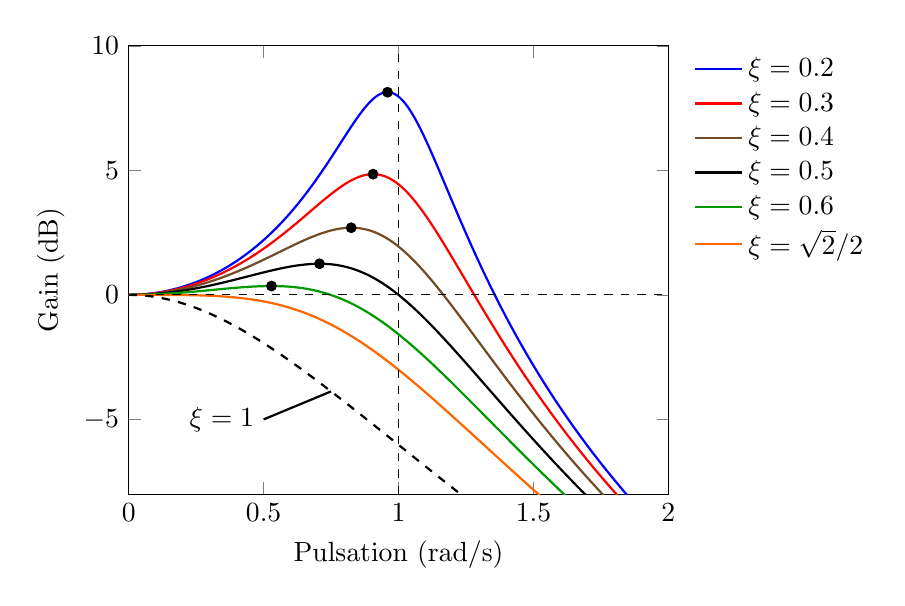
\begin{tikzpicture}
        \pgfplotscreateplotcyclelist{mycolorlist}{%
            blue\\%
            red\\%
            brown!60!black\\%
            black\\%
            green!60!black\\%
            red!60!yellow\\
            }
        \begin{axis}[
            ticklabel style = {font=\normalsize},
            legend style={draw=none},
            legend pos=outer north east,        
            legend cell align={left},
            ylabel={Gain (dB)},
            xlabel={Pulsation (rad/s)},
            xmode=normal,ymode=normal,
            xmin=0.0, xmax=2,
            ymin=-8, ymax=10,
            %grid=both,
            major grid style={black!40},
            cycle list name=mycolorlist,
        ]
        \foreach \a in {0.2,0.3,0.4,0.5,0.6,0.707}
            \addplot+[thick,domain=0:2, samples=501] {-20*log10(sqrt((1-x*x)^2 +(2*\a*x)^2 ))}; 
        \addplot[dashed,domain=0.1:5, samples=201] {0};
        \def\a{1.0}
        \addplot [dashed,thick,domain=0:2, samples=501] {-20*log10(sqrt((1-x*x)^2 +(2*\a*x)^2 ))}; 
        \coordinate (P) at (axis cs:0.75,{-20*log10(sqrt((1-0.75*0.75)^2 +(2*\a*0.75)^2 ))});
        \node[left] (a) at (axis cs:0.5,-5) {$\xi=1$};
        \draw [thick] (a.east) -- (P);
                \addplot[mark size=1.75pt,color = black,fill=black,mark=*,only marks] coordinates {
        	(0.959166304663,8.13608784305)
        	(0.905538513814,4.84656106912)
        	(0.824621125124,2.69540739954)
        	(0.707106781187,1.24938736608)
        	(0.529150262213,0.354575339209)
       	};
        \draw[dashed] (axis cs:1,-10) -- (axis cs:1,10);
            \legend{$\xi=0.2$,$\xi=0.3$,$\xi=0.4$,$\xi=0.5$,$\xi=0.6$,$\xi=\sqrt{2}/2$}
        \end{axis}
    \end{tikzpicture}
%    \caption{\'Evolution du gain en décibel en fonction de la pulsation pour différentes
%    valeur du taux d'amortissement du régime pseudo-périodique. Le gain maximal à la pulsation 
%    de résonance $\omega_r$ est représenté par une pastille noir sur chacune des courbes pour $\xi<\sqrt{2}/2$.
%    On remarquera l'utilisation exceptionnel d'une échelle linéaire pour les pulsations.}
\end{figure}

